\section{Architecture}
\label{sec:architecture}
% The architecture diagram: https://thehdfgroup-my.sharepoint.com/:u:/g/personal/mlarson_hdfgroup_org/EWdh_K7tOc5JhB0mJPSAJuYBzKx2uFQ5RvwqQQLdOyKxew?e=7T9Ngr

\subsection{Metadata Cache vs. Page Buffer}

As the WAL requires a client module that is responsible for handling metadata I/O to the file, it could be feasibly achieved with either the metadata cache or the page buffer as its primary client. For several reasons, we chose to pursue implementation via the metadata cache:

\begin{itemize}
    \item An implementation through the page buffer would necessitate either tracking which page sections are updated by writes, or writing exclusively entire metadata pages to the WAL. Tracking page sections would increase complexity greatly, and writing entire pages may negatively impact performance and increase the size of the WAL.
    
    \item The page buffer is often bypassed - for example, when an I/O operation is larger than one page. Implementing the WAL through the page buffer would require forcing all metadata to always pass through the page buffer.
    
    \item An implementation through the page buffer would still need to notify the metadata cache at the time of a log flush or log checkpoint (see \hyperref[sec:Flush-Types]{Flush Types}) in order to accurately satisfy later metadata reads. Implementing the WAL through the metadata cache means that this introduces no additional coupling.

\end{itemize}

\subsection{Flush Types}
\label{sec:Flush-Types}

There are two types of metadata flush that the library may perform:

\begin{enumerate}
    \item A "log flush" - Flushes metadata from the cache to the WAL file to create a self-consistent location to play forward to in the event of a crash.

    \item A "log checkpoint" - Replays metadata writes from the WAL to the HDF5 file to bring the file up-to-date with metadata operations until a specific point. This requires reading a WAL entry from the WAL file for each metadata write performed. This is the type of flush invoked by \texttt{H5Fflush()}.
\end{enumerate}

Each type of flush operation leaves a 'marker' in the WAL after the last WAL entry upon which it acts.

All WAL entries before a log checkpoint marker have already been written to the HDF5 file and may be safely trimmed from the WAL. A WAL trim operation involves truncating the WAL file so it only contains the WAL superblock, effectively deleting all WAL entries.

A complete implementation of the WAL without log checkpoint markers is possible, if the WAL is always trimmed immediately after each log checkpoint. In this case, all entries which would be placed before a log checkpoint marker are instead removed from the WAL entirely, and so the marker is not necessary to indicate that these entries should be skipped during subsequent WAL operations.

A log flush marker indicates that all WAL entries since the last log checkpoint should be 'played forward' to the HDF5 file during a log checkpoint or crash recovery. Log flush markers prevent re-execution of torn metadata writes, since if a torn write occurs during a log flush and leaves a malformed WAL entry, no log flush marker will be present and no modification of the HDF5 file will be attempted.

\subsection{Metadata Cache + WAL Lifecycle}
\label{sec:Metadata-Cache-WAL-Lifecycle}
In order to avoid high overhead from constant small batches of I/O, log checkpoints are performed at intermittent intervals based on either the passage of real time via a 'tick' system similar to the one proposed in the VFD SWMR RFC~\cite{rfc20180610}, or based on the quantity of metadata written to the file. The specific criteria for and frequency of log checkpoints during library operation is configurable by the application via property lists. Due to the partition of information between different layers of the library, specific user-provided values for intervals at which these operations act as heuristics rather than exact thresholds.

I/O to the WAL file uses the active VFD for the file, unless a different VFD is provided at the time the WAL is enabled by \texttt{H5P\_set\_wal()}. 

\subsubsection{Metadata Writes}

\begin{figure}
    \centering
    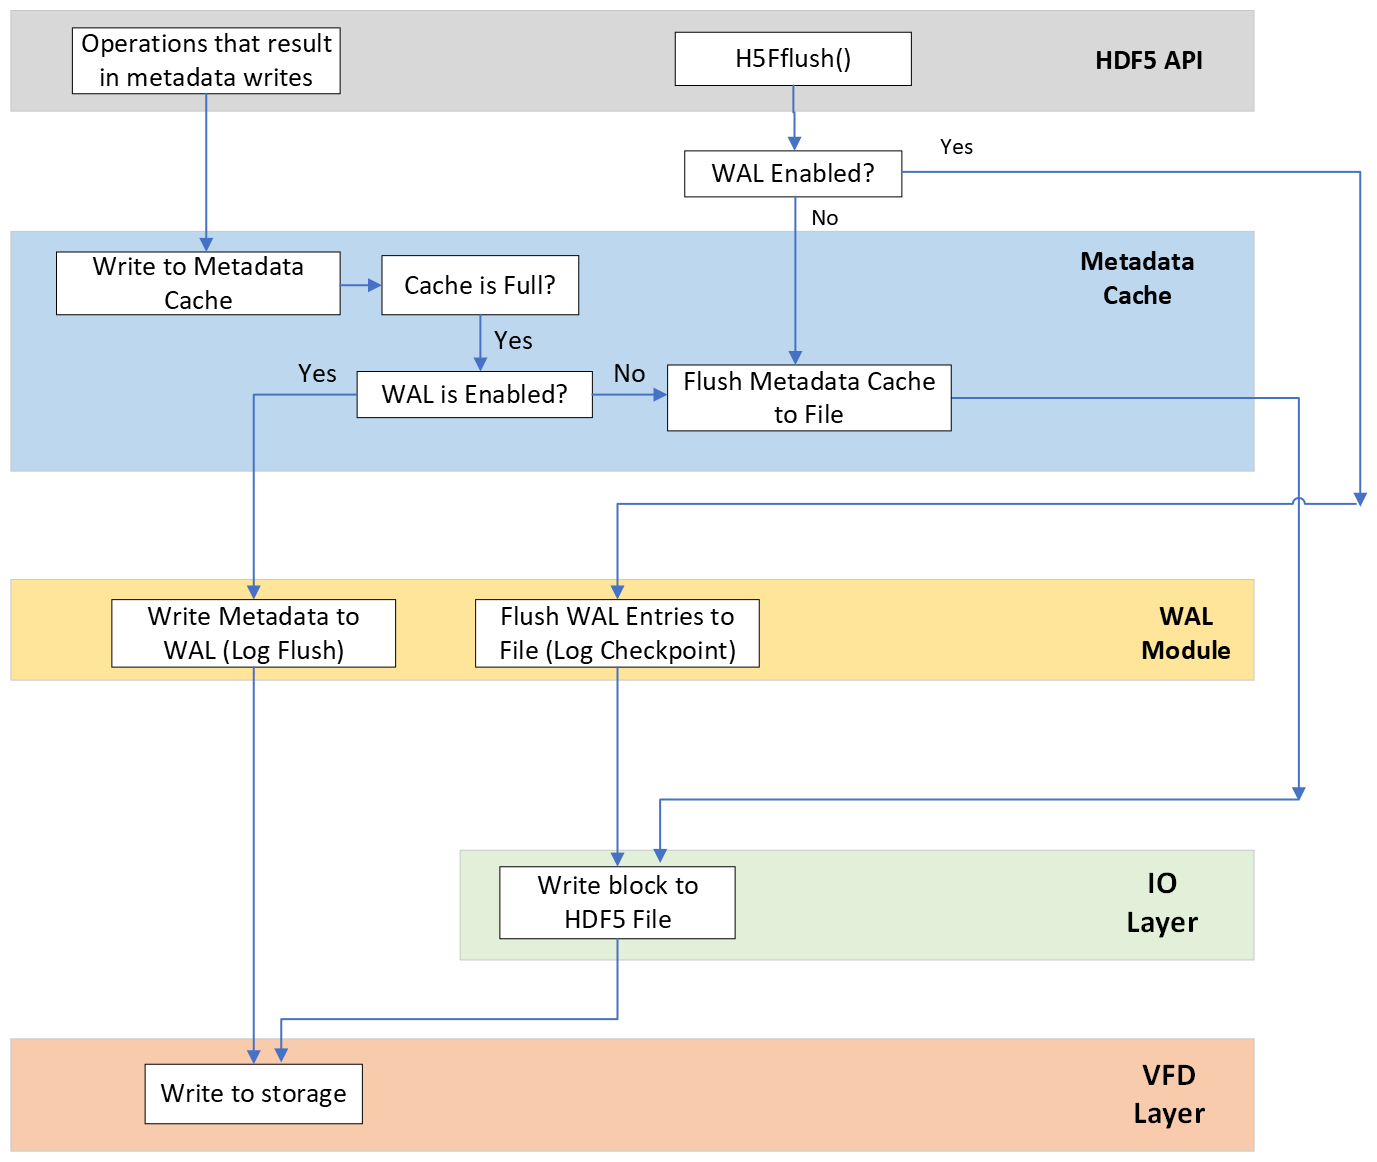
\includegraphics[width=1.0\textwidth]{images/wal_design.png}
    \caption{Overview of different types of metadata writes}
    \label{fig:wal-diagram}
\end{figure}

Figure~\ref{fig:wal-diagram} illustrates how the WAL alters the existing flow of metadata writes through the library.  Writes which do not prompt a flush of the metadata cache have no special handling with the WAL enabled. Once a metadata write prompts a cache flush, it will be performed as a log flush which writes metadata to the WAL file and leaves stub entries in the metadata cache. The metadata in WAL entries is not written to the HDF5 file until a log checkpoint, which is either directly invoked by \texttt{H5Fflush()} or invoked each time a user-defined threshold is reached.


\subsubsection{Metadata Reads}
The MDC must be able to read back WAL entries in order to correctly service read operations when the WAL contains a more recent version of a metadata object than the file (e.g. after a log flush but before a log checkpoint). When a dirty object is evicted from the cache, a 'stub' entry is left in the cache. This stub entry records the address of the WAL entry within the WAL file so that it may be quickly read at a later time.

The full process for a metadata read is as follows:
\begin{itemize}
    \item If the requested metadata object is not in the metadata cache, fulfill the read from the file.

    \item If the requested metadata object has a non-stub entry in the metadata cache, fulfill the read from the metadata cache.

    \item If the requested metadata object has a stub entry in the metadata cache, fulfill the read from the WAL entry. 
\end{itemize}

\subsection{Metadata Deletion and Raw Data Integrity}
\label{sec:Metadata-Deletion}

\begin{figure}
    \centering
    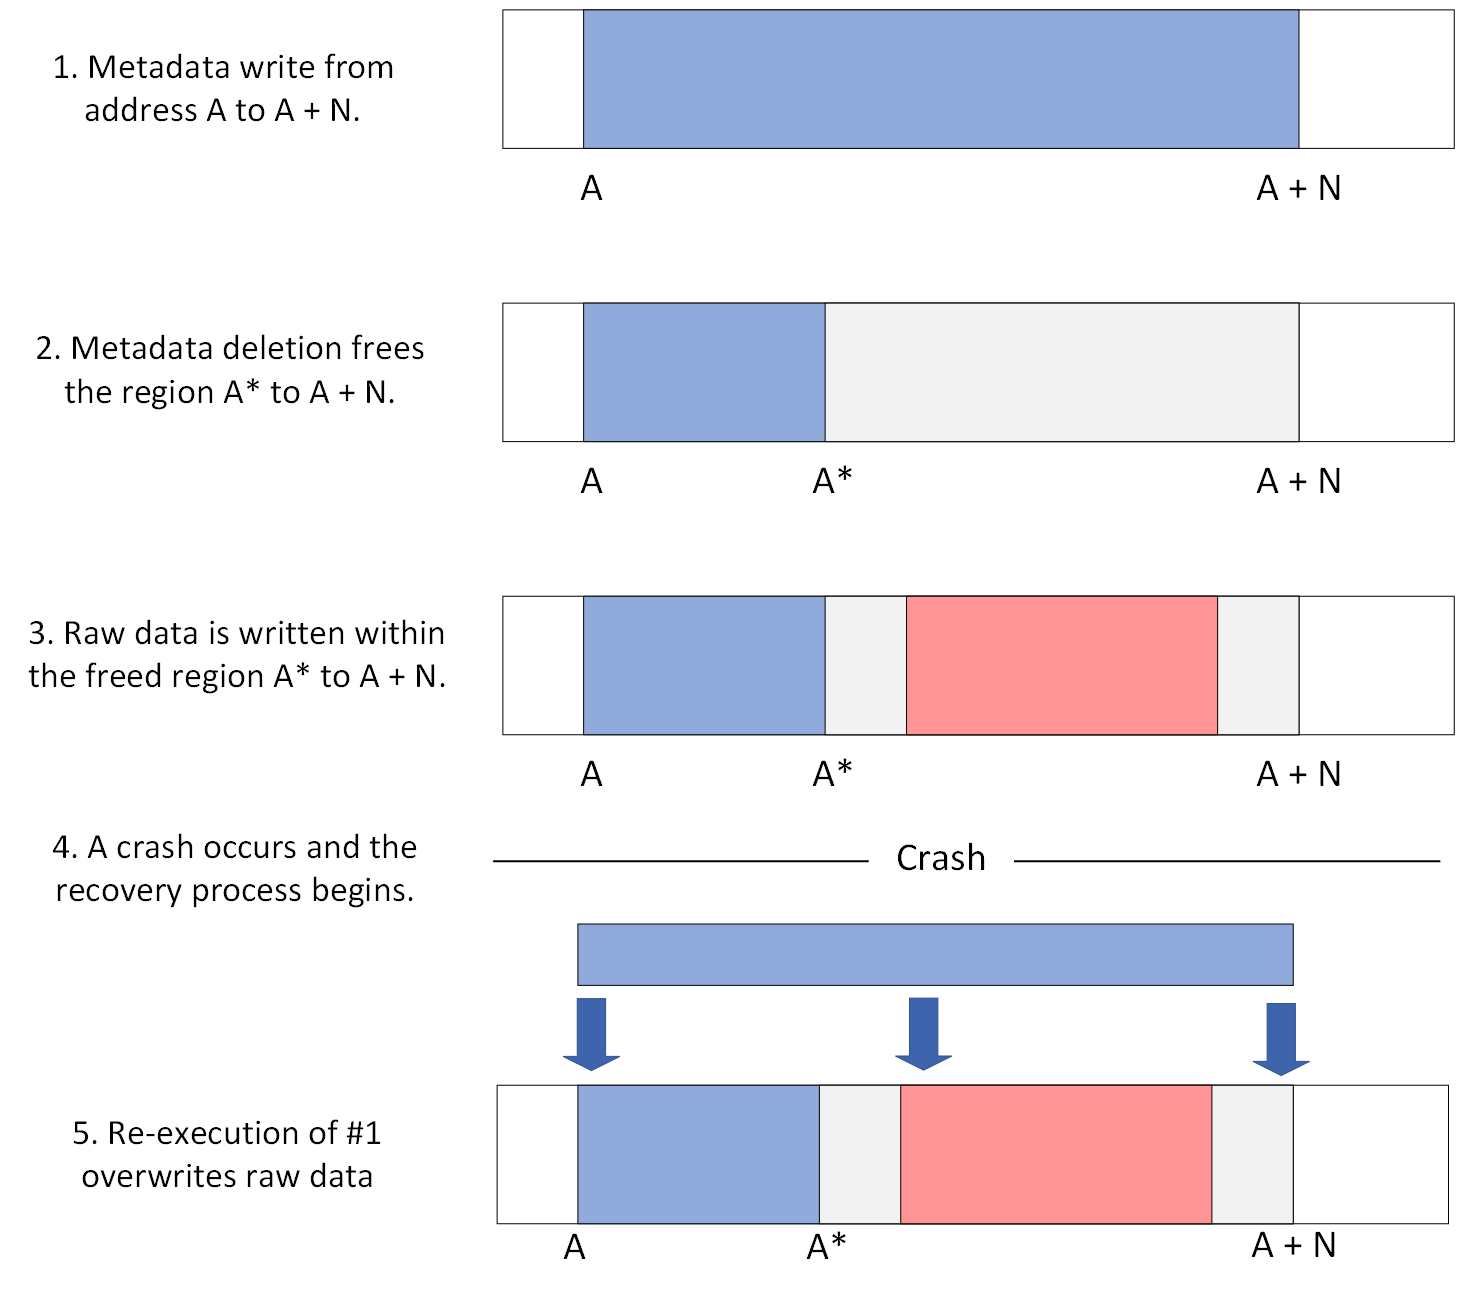
\includegraphics[width=1.0\textwidth]{images/wal_md_delete_diagram.png}
    \caption{A series of WAL operations that would result in raw data being overwritten during recovery}
    \label{fig:wal-md-delete-diagram}
\end{figure}

Consider the following series of events on a file with the WAL enabled, as illustrated in Figure~\ref{fig:wal-md-delete-diagram}:

\begin{enumerate}
    \item A user operation results in a metadata write to offset \texttt{A} of length \texttt{N} within the file. This write is logged to the WAL.
    
    \item A user operation results in the deletion of a section of metadata, \texttt{A*} to \texttt{A* + N*}, that resides entirely or partially within the address region \texttt{A} to \texttt{A + N}. 
    
    \item Due to free space recycling being enabled on the file, the region \texttt{A*} to \texttt{A* + N*} is marked as free for other usage within the library.

    \item A user operation results in raw data being written to the file in the (now free) region \texttt{A*} to \texttt{A* + N*}. Because this is a raw data operation, it bypasses the WAL.

    \item Before the next log checkpoint, a crash occurs.

    \item Crash recovery begins, and eventually executes the metadata write from event \#1. This results in the overwriting of whatever portion of the user's raw data was in the filespace range marked as free by event \#3, from \texttt{A*} to address \texttt{A* + N*}.
\end{enumerate}

    Strictly speaking, raw data integrity is outside the scope of the Write-Ahead Log, but it is still preferable to preserve the integrity of application data as much as possible in the event of a crash. 

    To prevent this potential loss of raw data, the preferred option is to defer recycling free space for metadata until the next log checkpoint. Metadata generally takes up a relatively small amount of space in the file compared to raw data, so the potential gains from optimizing space usage in this case are limited, especially given the algorithmic overhead required to enable it.

    If there exists a use case for which non-deferred metadata free space recycling is critical, the following is an outline of the changes necessary to support simultaneous raw data integrity and non-deferred metadata free space recycling:

    The WAL entry file format would need to be expanded to support dividing a metadata block into isolated sections. This is necessary because repeated metadata deletions could divide a previously contiguous block of metadata into an arbitrary number of distinct sections. Tracked information would need to include the quantity of sections, their lengths, and their offsets. In order to keep each WAL entry header a fixed size (to avoid fracturing writes), there would need to be a fixed upper bound on the potential number of sections within a single entry. 

    A rough sketch of an algorithm to track these metadata sections within WAL entries is as follows:
    
    \begin{enumerate}
        \item At the time of a metadata deletion, search the metadata cache for any metadata writes which overlap the deleted region and have not been written to the file. The metadata cache contains stub entries with the length and offset of the metadata, which allow this search to be done without a disk read.
        
        \item If any of the WAL entries with overlapping writes already have more than the maximum number of distinct sections, then trigger a log checkpoint of the WAL. After this, no previous metadata writes will need to be re-executed, so this process ends.

        \item For each WAL entry with a metadata block that overlaps the deleted metadata block, add one or more additional sections:
        
        \begin{enumerate}
            \item Determine which of its existing sections overlap the deleted region.

            \item For each section that overlaps the deletion, decrease its length so that no valid sections of the metadata section overlap the deleted region.

            \item If the deletion results in the creation of a new section within the block (e.g. if the deletion overlaps with a section, but not the end of that section), compute the length and start address of the new section.

            \item If this process would result in the creation of enough new sections in the metadata block to push the WAL entry over the maximum number of entries, then perform a log checkpoint instead.
        \end{enumerate}
    \end{enumerate}

\subsubsection{WAL Lifecycle}

The WAL file will be created and its superblock initialized at file open time if the WAL is enabled on the file access property list (FAPL) for the file open/create operation. The WAL will be deleted when the file is closed normally, or after recovery if the file was reopened with the WAL disabled.

\subsection{Compatibility with Other Library Features}

\subsubsection{Parallel HDF5}

WAL compatibility with Parallel HDF5 could be achieved by designating a single process as the WAL writer, and having all I/O to the WAL be performed through that process. 

Due to how parallel HDF5 handles each rank's metadata cache, additional synchronization points between the ranks will not be necessary for WAL compatibility. Because metadata writes must be done collectively, each rank will have the same dirty metadata cache entries to be flushed at the same time. Each rank will create a stub entry containing the target address in the WAL file, but only the designated writer will actually perform the write to the WAL file. Each rank will have up-to-date read access to the WAL file without additional work or I/O.

Because each process needs to be able to read directly from the WAL, the WAL file must be exposed to all processes in a similar manner to the HDF5 file itself. In order to maintain consistency, there will be an additional requirement that all ranks use the same log flush and log checkpoint intervals, and these intervals must be based on bytes written. In this way every process will have the same understanding of when log flushes and log checkpoints occur, and thereby will know when to eliminate stub entries.

\subsubsection{SWMR (Single Writer/Multiple Reader)}

There are multiple ways to enable SWMR access with crashproofing enabled. Perhaps the simplest method would be for the SWMR readers to ignore the WAL file and only look at the HDF5 file. This would of course prevent them from seeing any updates until a log checkpoint. Correct ordering of writes when replaying the WAL during the log checkpoint should happen naturally since the existing SWMR mechanism will have correctly ordered the writes in the WAL file, and they are replayed in that order.

Alternatively, we may wish for the readers to be aware of the WAL file and scan it for updates to metadata. They could either only look at WAL entries up to the latest log flush marker, or look at all entries. In either case we would want to be careful to handle the case where a log checkpoint occurs during a SWMR read operation. The need to avoid caching information about the location of metadata in the WAL would necessitate scanning the WAL frequently, which may make the first approach more feasible.

\subsubsection{Page Buffer}

Because the WAL largely replaces metadata writes to the HDF5 file with writes to the WAL file, the page buffer is less relevant than when not using the WAL. That said, we may be able to achieve a similar effect on writes by, when flushing multiple entries to the WAL (at log flush time or otherwise), assembling WAL entries into a single buffer before writing them to the WAL in a single operation. It should also be possible to use the page buffer only at log checkpoint time to perform metadata writes in larger blocks, though this will only benefit the log checkpoint and file close operations.

In the future it will be possible to implement a page buffer like scheme for the WAL itself, which will aid in prefetching entries that exist only in the WAL, but this will not be in the initial implementation.

The standard HDF5 page buffer will still be available for use with raw data when the WAL is active, since the WAL does not modify the I/O pattern for raw data.

\subsubsection{Metadata Accumulators}

Metadata accumulators sit below the metadata cache and group small metadata I/O requests into larger batches to improve performance. Simultaneous use of the metadata accumulators and the WAL is not possible with the current design.

If an accumulator worked simultaneously with the WAL, then what the metadata cache considers distinct writes to the WAL file from distinct cache entries could be grouped into a single I/O request at the VFD layer. This would write a single WAL entry with a metadata block that contains metadata blocks from distinct metadata cache entries. At metadata read time, if a stub entry in the cache is used to read metadata from the WAL file, the metadata block retrieved would be larger than expected. While it would contain the requested metadata block, the metadata cache lacks the capabilities to perform introspection on the accumulated metadata block to determine which region has the requested data. 

As log checkpoints involve no writes to the WAL file, metadata accumulators may be used during log checkpoint operations, with the constraint that the accumulator be flushed afterwards. Since this would provide little to no opportunity for the accumulator to bundle I/O requests, the potential usefulness of enabling the accumulators for this case is debatable.


\subsubsection{Variable-Length and Reference Datatypes}

Variable-length and reference datatypes require special consideration, since the 'raw data' for these types has a metadata component. Data with a variable-length or reference datatype is written to file as global heap IDs which point to the location of the actual data within the file's global heap (i.e. within the metadata portion of the file).

As the metadata cache does not draw a distinction between metadata for these types and 'regular' metadata, the most straightforward solution is to treat these metadata operations in the same manner as other metadata writes. 

Because the amount of data in variable-length and reference datasets is likely to be much higher than other kinds of metadata, using these datatypes extensively will likely increase the I/O and storage overhead of the WAL. Therefore, we may decide to add an option to exclude these types of objects from the WAL and remove consistency guarantees for variable length and reference data.

\subsubsection{Compact Datasets}

Compact datasets store the dataset's raw data within the object header. Just like variable-length and reference datatypes, this results in what the application views as raw data being stored and retrieved as metadata. As in that case, because the semantic meaning of the metadata block is not known to the metadata cache, the WAL will treat metadata describing a compact dataset in the same manner as all other metadata.

Unlike for variable-length and reference datatypes, the size of compact datasets is strictly bounded, so it is unlikely that any option to disable the WAL for compact datasets will be added.

\subsection{WAL File Format}

\begin{figure}
    \centering
    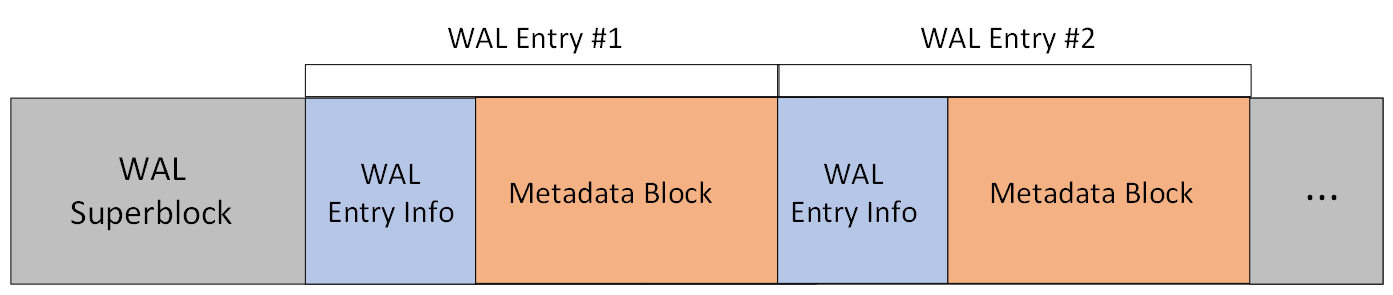
\includegraphics[width=1.0\textwidth]{images/wal_layout.png}
    \caption{The on-disk layout of a WAL file}
    \label{fig:wal-layout}
\end{figure}

The WAL file is composed of the WAL superblock and a contiguous series of WAL entries. A WAL entry consists of a WAL entry info block and a metadata block.

Reading an arbitrary WAL entry requires iterating through all prior WAL entries, but this is only done at log checkpoint and recovery time. Reads during log flushes are expedited by using stub entries in the metadata cache to jump directly to the address of the desired WAL entry. The speed of recovery is not a critical concern, as recovery is expected to be infrequent.

The WAL superblock consists of the following elements:

\begin{itemize}
    \item \texttt{version} - The version of the WAL file format in use.

    \item \texttt{filepath} - Filepath indicating the HDF5 file that this WAL corresponds to.

\end{itemize}

\subsubsection{WAL Entries}

Each WAL entry consists of a WAL entry info block, followed by the block of metadata for the logged metadata write. The fields in the WAL entry info block are as follows:

\begin{itemize}

\item \texttt{target\_offset} - The target offset in the HDF5 file for the metadata write operation. This field has two 'magic values' which indicate this this WAL entry is a marker. A log flush marker indicates that all previous entries are safe to be replayed in the event of a crash. A log checkpoint marker indicates that all previous entries have already been flushed to the file and do not need to be replayed. As mentioned earlier, we may eliminate log checkpoint markers in favor of always trimming the WAL on a log checkpoint, in which case the start of the WAL functions as an implicit log checkpoint marker. Markers do not contain any of the other fields listed below. Markers are stored in this fashion to avoid allocating space in each entry for a field that the majority of WAL entries will not use.

\item \texttt{length} - The size in bytes of this entry's metadata block.

\end{itemize}

We may also decide to add a checksum for the WAL entry info, or the metadata block, or both, though the metadata block may already be checksummed using existing HDF5 facilities so that may not be necessary.

WAL entries do not need start or end tags to avoid executing WAL entries that result from torn writes, because interrupted WAL entries are already handled by log flush markers. During recovery, the WAL is only played back until the most recent log flush marker. If the library terminates unexpectedly, any torn writes to the WAL will be after the most recent log flush marker, and thus will not be re-executed.

Most database implementations of a Write-Ahead-Log uniquely assign each log entry a monotonically increasing log sequence number. At the present stage, the HDF5 WAL would have no use for such a feature beyond potential consistency checks. The HDF5 WAL is not currently planned to support multiple simultaneous writers, removing a large motivation for the log sequence number. Finally, because the WAL file format is not intended to be future-proof in the same manner as the HDF5 file format, adding a log sequence number in a subsequent version if the need arises will be relatively painless. 

This design places the marker for log flushes/log checkpoints within individual WAL entries via a magic value in the 'offset' field. Another potential option is to store the marker in the WAL superblock as the offset of the latest WAL entry that has been log flushed/log checkpointed. This would have the advantage of improving recovery time, because storing markers in individual entries requires a preliminary scan of the entire WAL to determine which entries to replay. However, this would incur a performance penalty  by adding a  WAL header write to log flushes and log checkpoints.

\subsection{Additions to the API}

\begin{itemize}
    \item \texttt{herr\_t H5Pset\_wal(hid\_t fapl\_id,} \\
    \texttt{ const char *wal\_path,} \\
    \texttt{ H5WLinterval\_type\_t log\_flush\_interval\_type,} \\
    \texttt{ size\_t log\_flush\_interval,} \\
    \texttt{ H5WLinterval\_type\_t log\_checkpoint\_interval\_type,} \\
    \texttt{ size\_t log\_checkpoint\_interval,} \\
    \texttt{ hid\_t wal\_fapl\_id)} \\
    Modifies the file access property list \texttt{fapl\_id} to log metadata writes to a WAL file at \texttt{wal\_path}. \texttt{log\_flush\_interval\_type} determines which metric is used to initiate periodic log flush execution (bytes written, time, or none) and the value for that threshold is \texttt{log\_flush\_interval}. \texttt{log\_checkpoint\_interval\_type} determines which metric is used to initiate periodic log checkpoint execution (bytes written, time, or none) and the value for that threshold is \texttt{log\_checkpoint\_interval}. \texttt{wal\_fapl\_id} is a file access property list which is used to determine which VFD is used to perform I/O to the WAL file. If this parameter is \texttt{H5I\_INVALID\_HID}, the active VFD from \texttt{fapl\_id} is used for WAL file I/O.

    \item \texttt{herr\_t H5Pget\_wal(hid\_t fapl\_id,} \\
    \texttt{ const char **wal\_path,} \\
    \texttt{ H5WLinterval\_type\_t *log\_flush\_interval\_type,} \\
    \texttt{ size\_t *log\_flush\_interval,} \\
    \texttt{ H5WLinterval\_type\_t *log\_checkpoint\_interval\_type,} \\
    \texttt{ size\_t *log\_checkpoint\_interval,} \\
    \texttt{ hid\_t *wal\_fapl\_id)} \\
    Retrieves whether a given file access property list has the WAL enabled, the path to the WAL file if so, and the thresholds types and values for when log checkpoints are performed. If \texttt{*wal\_path} is returned as NULL then the WAL is disabled for the file.

    \item \texttt{herr\_t H5Pset\_wal\_auto\_recovery((hid\_t fapl\_id,} \\
    \texttt{bool enable\_auto\_recovery)} \\
    Determines whether, if a valid WAL path is detected at file open time (indicating a library crash) the metadata recovery process will automatically begin. 

    \item \texttt{herr\_t H5Pget\_wal\_auto\_recovery((hid\_t fapl\_id,} \\
    \texttt{bool *enable\_auto\_recovery)} \\
    Retrieves whether automatic metadata recovery on file open is enabled.

    \item \texttt{herr\_t H5Fwal\_flush(hid\_t file\_id)} \\
    Performs a log flush to the WAL. A counterpart to \texttt{H5Fflush()}, which performs a log checkpoint.
\end{itemize}


\subsection{The Recovery Process}

If WAL usage is enabled for a file, then recovery takes place at file open time if the file did not close properly. Whether the file was closed properly is tracked in the HDF5 superblock, similar to the "journal open" flag from the Metadata Journaling RFC. It is tracked via a superblock message containing the filepath of the WAL file.

At file open, this message is written, and it is deleted only at the end of the file closing process. Any premature termination of the library or an application using the library will leave the message in the superblock, which can be detected at file open time. 
        
The process to restore a file's metadata to a self-consistent state is as follows:

\begin{itemize}
    \item Scan the WAL from the beginning to the end to find both the most recent log checkpoint marker and the most recent log flush marker.
    \item Starting from the most recent log checkpoint marker  in the WAL (or from the beginning if there are none), read each WAL entry. Copy each entry's block of metadata to the specified offset in the file.
    \item When the recovery algorithm reaches the most recent log flush marker, stop processing any further WAL entries.
    \item Trim the WAL if the file was opened with WAL enabled. If the file was opened with the WAL not enabled, delete the WAL file and remove the HDF5 superblock message.
\end{itemize}

If a file was not closed cleanly and is reopened with read only access, the recovery process is different:

\begin{itemize}
    \item Scan the WAL from the beginning to the end to find both the most recent log checkpoint marker and the most recent log flush marker.
    \item Starting from the most recent log checkpoint marker in the WAL (or from the beginning if there are none), read each WAL entry. Create a stub entry in the cache for each WAL entry.
    \item When the recovery algorithm reaches the most recent log flush marker, stop reading any further WAL entries.
\end{itemize}

Depending on available resources, we may delay implementation of the read only reopen case.